\documentclass[11pt]{article}
\usepackage{subfigure,wrapfig,graphicx,booktabs,fancyhdr,amsmath,amsfonts}
\usepackage{bm,amssymb,amsmath,amsthm,wasysym,color,fullpage,setspace,multirow}
\newcommand{\vb}{\boldsymbol}
\newcommand{\vbh}[1]{\hat{\boldsymbol{#1}}}
\newcommand{\vbb}[1]{\bar{\boldsymbol{#1}}}
\newcommand{\vbt}[1]{\tilde{\boldsymbol{#1}}}
\newcommand{\vbs}[1]{{\boldsymbol{#1}}^*}
\newcommand{\vbd}[1]{\dot{{\boldsymbol{#1}}}}
\newcommand{\vbdd}[1]{\ddot{{\boldsymbol{#1}}}}
\newcommand{\by}{\times}
\newcommand{\tr}{{\rm tr}}
\newcommand{\cpe}[1]{\left[{#1} \times \right]}
\newcommand{\sfrac}[2]{\textstyle \frac{#1}{#2}}
\newcommand{\ba}{\begin{array}}
\newcommand{\ea}{\end{array}}
\renewcommand{\earth}{\oplus}
\newcommand{\sinc}{{\rm \hspace{0.5mm} sinc}}
\newcommand{\tf}{\tilde{f}}
\newcommand{\tbox}[1]{\noindent \fbox{\parbox{\textwidth}{#1}}}
\DeclareMathAlphabet{\mathpzc}{OT1}{pzc}{m}{it}

\title{ASE 379L Laboratory 1 Report \\ Simulating Quadrotor Dynamics}
\author{Susan Burling Ward} \date{February 5, 20XX}

\begin{document}
%\onehalfspace
\maketitle
\section{Abstract} \emph{The abstract is a summary of the whole report.  Out
  of respect for our busy readers, it gets right to the point.  The first 2-3
  sentences unpack the title and motivate the report.  The remainder briefly
  offer context (if necessary) and describe the reports's method and
  main results.} \\

A high-fidelity quadrotor dynamics simulator was designed from the theory of
Newtonian dynamics and then implemented in Matlab code ...

\section{Introduction} \emph{Put here a brief introduction to the lab's
theme. Refer to relevant papers from our readings, or other papers you have
found.  This introduction need not be long: 2 paragraphs should be adequate.}\\

Quadrotor motion can be described by a combination of linear and attitude
dynamics and certain linear motion and attitude kinematics relationships.  The
governing equations for a simplified simulator can be found in
\cite{mellinger2012trajectory}.  However, a high-fidelity simulator must
account for effects that \cite{mellinger2012trajectory} ignores ...

\section{Theoretical Development} \emph{Put here any theoretical development (e.g.,
modeling) required to answer the boxed questions posed in the lab assignment.
Then proceed to answer the theoretical boxed questions from the lab---those
that do no depend on experimental results.}

\section{Implementation} \emph{Describe here your basic implementation strategy and
any non-obvious implementation aspects.  Include snippets of your code
here to illustrate its features.  Put the complete code in an Appendix to the
lab report.}

\section{Results and Analysis}
\emph{Perform all tests and experiments requested by the lab, and analyze the
  results of these experiments. Answer any remaining boxed questions that were
  not answered in the Theoretical Development section.}\\

The {\tt simulateQuadrotorDynamics} function was run on the three input
structures {\tt Stest} provided.  The simulated attitude and position of the
quad for each of these is shown in Figs. \ref{fig:sca} and
\ref{fig:utdata}. ...

\begin{figure}[ht]
\begin{center}
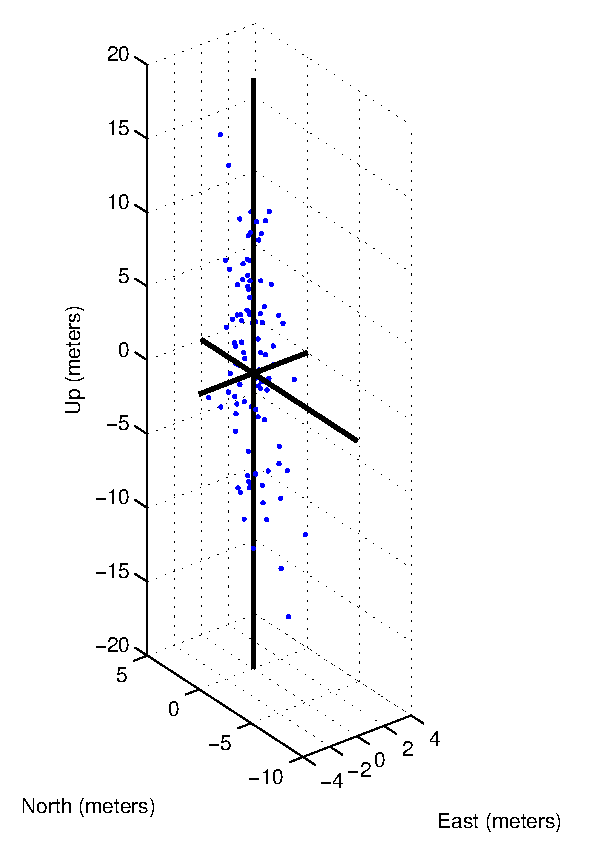
\includegraphics[width=0.4\textwidth]{figs/sca2.eps}
\end{center}
\caption{Quad attitude expressed as a time series of Euler angles.}
\label{fig:sca}
\end{figure}

\begin{figure}[ht]
\begin{center}$
\begin{array}{ccc}\hspace{-5em}
 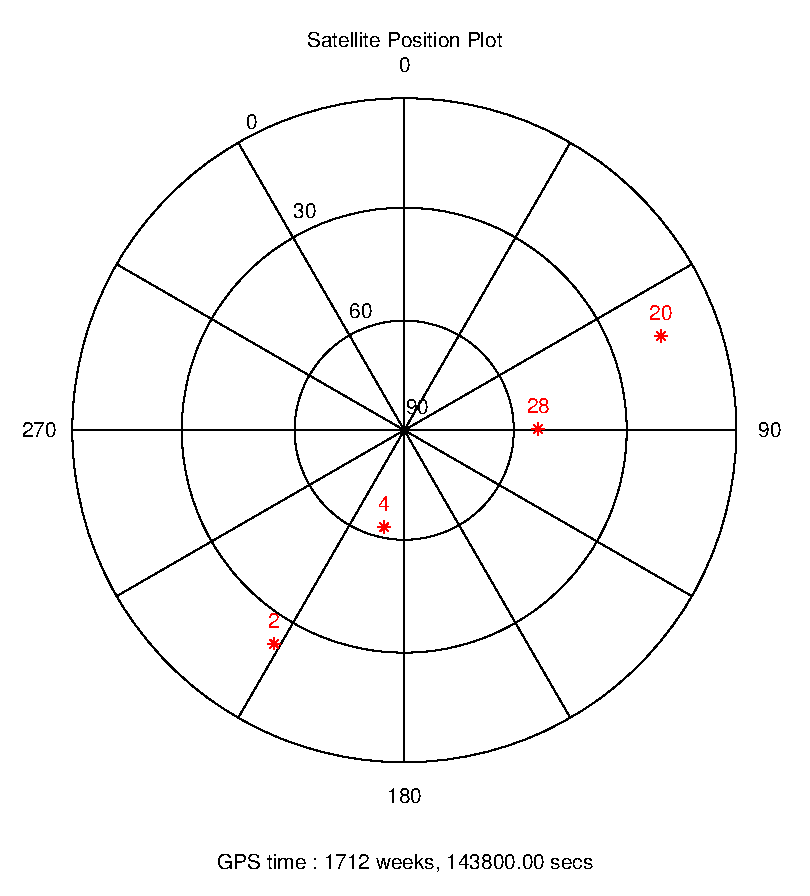
\includegraphics[width=0.4\textwidth]{figs/sky1.eps} &
 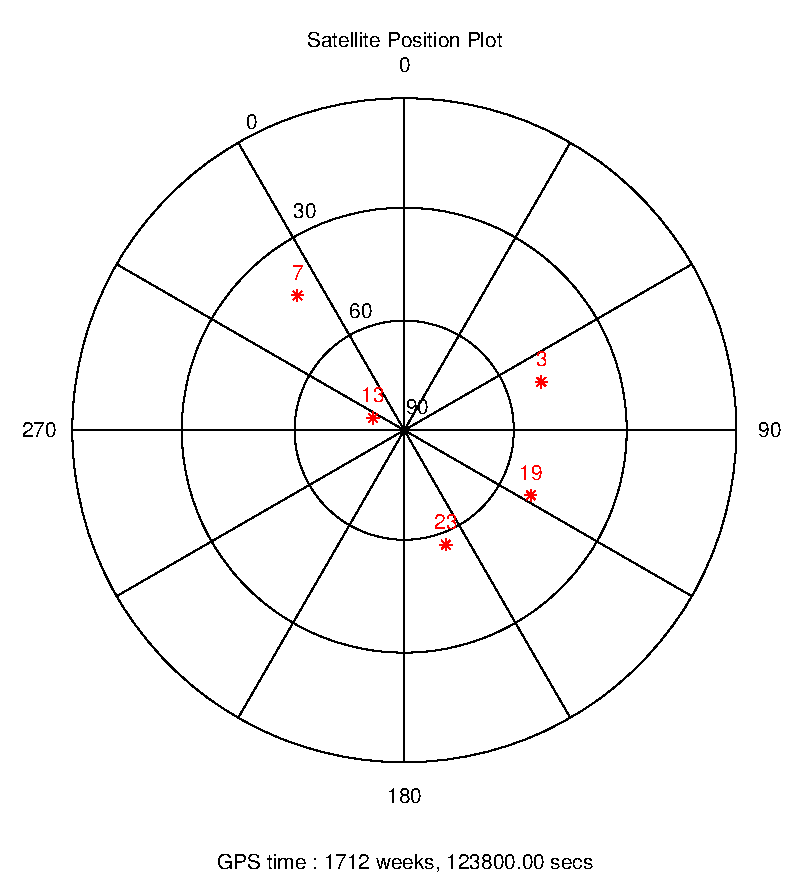
\includegraphics[width=0.4\textwidth]{figs/sky2.eps}
\end{array}$
\end{center}
\caption{[Figure caption here]}
\label{fig:utdata}
\end{figure}

Table \ref{tab:Chi2Fits} below shows...

\begin{table}[h!]
\begin{center}
    \begin{tabular}[c]{cccc}
    \toprule
    Data Source &  Sets, DOF & Nakagami-m & Rice \\ \midrule
    Wideband UHF & 79, ~~8 & 11.8 $\pm$ 8.8 & 9.0 $\pm$ 4.3 \\
    GPS L$_1$ & 33, ~~7 & 8.42 $\pm$ 5.9 & 7.7 $\pm$ 5.7 \\ \bottomrule
  \end{tabular}
  \label{tab:Chi2Fits}
  \caption{[Table caption here.]}
  \end{center}
\end{table}

\emph{Further analyze the results here.}

\section{Conclusion}
\emph{Much like the abstract, the Conclusion summarizes the most important
  results of the report.  It should be fairly short (one paragraph) and to the
  point.} \\

An open-loop control strategy was developed to generate the rotor
angular rates required to cause the simulated quadcopter to fly in a complete
circle on a horizontal plane.  The strategy was based on ...

\bibliographystyle{ieeetr}
\bibliography{./pangea}  
\end{document}
